\chapter{Pembahasan}

%=========================================================%
%               TULIS ISI PEMBAHASAN DI SINI              %
% Jangan Lupa untuk Menghapus Contoh Tulisan di Bawah Ini %
%=========================================================%

Ini adalah inti dari makalah Anda, tempat Anda menyajikan dan menganalisis data atau argumen Anda.

\textbf{Penyajian Data:} Sajikan data atau hasil riset Anda secara sistematis. Gunakan tabel, grafik, atau diagram untuk memvisualisasikan data agar lebih mudah dipahami.

\textbf{Analisis Temuan:} Analisis data yang telah disajikan. Hubungkan temuan Anda dengan teori-teori yang telah Anda paparkan di Kajian Pustaka. Jelaskan mengapa data tersebut muncul, apa artinya, dan apa implikasinya terhadap topik yang Anda teliti.

\textbf{Diskusi:} Bandingkan temuan Anda dengan hasil dari penelitian terdahulu. Apakah temuan Anda mendukung atau membantah penelitian sebelumnya? Diskusikan juga keterbatasan dari penelitian Anda dan kemungkinan faktor-faktor lain yang mungkin memengaruhi hasil.

\section{\textit{Formatting} Tulisan}

\subsection{Jenis \textit{Font}}

\begin{enumerate}[label=\alph*.]
    \item \textbf{\textit{Serif} (\textit{Main Font})}. \textit{Font} ini langsung digunakan saat Anda mengetikkan tulisan biasa. Sama saja dengan \verb|\text{TEKS}|. \\
    \texttt{OUTPUT} $\rangle$ Ketik apa pun, hasilnya akan menjadi begini.
    \item \textbf{\textit{Sans-Serif}}. \textit{Font} ini dapat digunakan dengan perintah \verb|\textsf{TEKS}|. \\
    \texttt{OUTPUT} $\rangle$ \textsf{Ini \textit{font sans-serif}. Kelihatan kan bedanya!}
    \item \textbf{\textit{Monospace}}. Font ini dapat digunakan dengan perintah \verb|\texttt{TEKS}|. \\
    \texttt{OUTPUT} $\rangle$ \texttt{Ini font monospace. Mirip dengan font kode.}
\end{enumerate}

\subsection{\textit{Font Style}}

\begin{enumerate}[label=\alph*.]
    \item \textbf{Normal}. Hanya tulisan normal.
    \item \textbf{\textit{Bold}/Tebal}. Dapat digunakan dengan menekan CTRL + B dalam \TeX\ Studio atau dengan perintah \verb|\textbf{TEKS}|. \\
    \texttt{SAMPLE} $\rangle$ Sebagian teks ada yang \textbf{tebal}.
    \item \textbf{\textit{Italic}/Miring}. Dapat digunakan dengan menekan CTRL + I dalam \TeX\ Studio atau dengan perintah \verb|\textit{TEKS}|. \\
    \texttt{SAMPLE} $\rangle$ Sebagian teks ada yang \textit{miring}.
    \item \textbf{\textit{Underline}/Bergaris Bawah}. Dapat digunakan dengan mengeklik \underline{U} dalam \TeX\ Studio atau dengan perintah \verb|\textbf{TEKS}|. \\
    \texttt{SAMPLE} $\rangle$ Sebagian teks ada yang \underline{digarisbawahi}.
    \item \textbf{\textit{Superscript}}. Dapat digunakan dengan dengan perintah \verb|\textsuperscript{TEKS}|. Jangan gunakan tombol $x^2$ atau perintah \verb|^{TEKS}| jika bukan untuk matematika. \\
    \texttt{SAMPLE} $\rangle$ Maaf. Kami hanya orang \textsuperscript{kecil}.
    \item \textbf{\textit{Subscript}}. Dapat digunakan dengan dengan perintah \verb|\textsubscript{TEKS}|. Jangan gunakan tombol $x_2$ atau perintah \verb|_{TEKS}| jika bukan untuk matematika. \\
    \texttt{SAMPLE} $\rangle$ Maaf. Kami hanya orang \textsubscript{kecil}.
\end{enumerate}

\section{Teks Matematika (\textit{Math Mode})}

Anda bisa menuliskan teks matematika untuk matematika biasa atau fisika. Sebagai catatan, Anda dapat menemui suatu aturan yang menyarankan beberapa notasi untuk jangan ditulis miring, sebab notasi bertulis miring diartikan sebagai variabel. Jika terjadi saat di dalam \textit{math mode}, dapat diatasi dengan:

\begin{enumerate}[nosep]
    \item Mencobai perintah yang tersedia seperti \verb|\det|, \verb|\sin|, \verb|\cos|, \verb|\tan|, dan lain sebagainya;
    \item Menambahkan \verb|up| sebelum nama notasi --- seperti \verb|\pi| menjadi \verb|\uppi|;
    \item Membungkus notasi menggunakan \verb|\mathrm{NOTASI}|, atau;
    \item Membungkus notasi menggunakan \verb|\text{NOTASI}|.
\end{enumerate}

Beberapa notasi yang harus diperhatikan untuk tidak ditulis miring dapat dilihat pada \autoref{table:notasi-tegak}.

\begin{table}[H]
    \centering
    \caption{Notasi yang Disarankan untuk Ditulis Tegak}
    \label{table:notasi-tegak}
    \begin{tblr}{colspec={l l}, hline{1,2,Z}={1-Z}{1pt, solid}}
        Kategori & Contoh Penulisan yang Disarankan \\
        Konstanta & $\mathrm{e} \quad \mathrm{i} \quad \uppi \quad \upphi \quad \uptau \quad \dots$ \\
        Himpunan Bilangan & $\mathbb{N} \quad \mathbb{Z} \quad \mathbb{Q} \quad \mathbb{R} \quad \mathbb{C} \quad \dots$ \\
        Operator & $\mathrm{d} \quad \mathrm{d}y \quad \mathrm{d}x \quad \mathrm{e} \quad \mathrm{e}^x$ \\
        Nama Operator & $\det \quad \mathrm{adj} \quad \mathrm{mod} \quad \log \quad \ln \quad \lim \quad \sin \quad \cos \quad \tan \quad \dots$ \\
        Satuan/Unit & $1\mathrm{m} \quad 2\mathrm{s} \quad 3\mathrm{kg} \quad 4\mathrm{A} \quad 5\mathrm{K} \quad 6\mathrm{J} \quad 7\mathrm{N} \quad 8\Omega \quad \dots$ \\
        Keterangan & $\mathrm{maks} \quad x_{\mathrm{awal}} \quad x_{\mathrm{akhir}} \quad 2^{\text{banyaknya peserta}} \quad \mathrm{damage} \times 3 \quad \dots$
    \end{tblr}
\end{table}

Sebagian contoh notasi bertulis tegak yang ditunjukkan pada \autoref{table:notasi-tegak} bukanlah suatu paksaan. Hal tersebut kembali lagi pada aturan/kemauan sang tutor. Jika tutor Anda tidak mempermasalahkan ini, maka Anda tidak perlu pusing dengan aturan ini.

\subsection{\textit{Inline Math} (Ditulis Sebaris dengan Teks)}

\begin{enumerate}[label=\alph*.]
    \item \textbf{\textit{Keep it Inline Style}}. Teks matematika ditampilkan lebih kecil agar tetap pas dengan baris-baris dalam paragraf. Anda dapat menggunakannya dengan perintah \verb|\(...\)| atau \verb|$...$|, bagian $\dots$ diisikan dengan kode matematika \LaTeX.
    
    Misalnya kita punya pecahan $y = \frac{ax + b}{cx + \sqrt{d}}$, lalu integral $\int_{a}^{b} f(x) \,\mathrm{d}x$, lalu ekspresi matematika $\sum_{i=1}^{n} i^2 = \frac{n(n+1)(2n+1)}{6}$, dan limit $\lim_{x \to 0} \frac{\sin x}{x} = 1$
    
    \item \textbf{\textit{Inline with Display Style}}. Teks matematika ditampilkan dengan ukuran aslinya. Anda dapat menggunakannya dengan perintah \verb|$\displaystyle ...$|, bagian $\dots$ diisikan dengan kode matematika \LaTeX.
    
    Misalnya kita punya pecahan $\displaystyle y = \frac{ax + b}{cx + \sqrt{d}}$, lalu integral $\displaystyle \int_{a}^{b} f(x) \,\mathrm{d}x$, lalu ekspresi matematika $\displaystyle \sum_{i=1}^{n} i^2 = \frac{n(n+1)(2n+1)}{6}$, dan limit $\displaystyle \lim_{x \to 0} \frac{\sin x}{x} = 1$
\end{enumerate}

\subsection{\textit{Display Math} Satu Baris}

\begin{enumerate}[label=\alph*.]
    \item \textbf{Polosan}. Gunakan perintah \verb|\[...\]|, bagian $\dots$ diisikan dengan kode matematika \LaTeX.
    
    Definisi turunan suatu fungsi $y = f(x)$ dengan notasi Leibniz (yang mengindikasikan perubahan infinitesimal) dirumuskan sebagai:
    \[\frac{\mathrm{d}y}{\mathrm{d}x} = \lim_{\Delta x \to 0} \frac{\Delta y}{\Delta x} = \lim_{\Delta x \to 0} \frac{f(x + \Delta x) - f(x)}{\Delta x}\]
    Ada pula definisi turunan lain yang lebih dikenal. Definisi turunan suatu fungsi $f(x)$ di titik $x$ adalah:
    \[f'(x) = \lim_{h \to 0} \frac{f(x+h) - f(x)}{h}\]
    
    \item \textbf{Bernomor \& Dapat Ditunjuk}. Gunakan \textit{environment} \texttt{equation} dan tambahkan \verb|\label| di akhir seperti:
    
    \begin{lstlisting}
        \begin{equation}
            TULISAN_MATEMATIKA_LATEX \label{eq:KATA_TUNJUK}
        \end{equation}    
    \end{lstlisting}
    
    Definisi turunan suatu fungsi $y = f(x)$ dengan notasi Leibniz (yang mengindikasikan perubahan infinitesimal) dirumuskan sebagai:
    \begin{equation}
        \frac{\mathrm{d}y}{\mathrm{d}x} = \lim_{\Delta x \to 0} \frac{\Delta y}{\Delta x} = \lim_{\Delta x \to 0} \frac{f(x + \Delta x) - f(x)}{\Delta x} \label{eq:derivatif-leibniz}
    \end{equation}
    Ada pula definisi turunan lain yang lebih dikenal. Definisi turunan suatu fungsi $f(x)$ di titik $x$ adalah:
    \begin{equation}
        f'(x) = \lim_{h \to 0} \frac{f(x+h) - f(x)}{h} \label{eq:derivatif-biasa}
    \end{equation}
    Sekarang kita coba tunjuk. Bisa dilihat pada \autoref{eq:derivatif-leibniz} bahwa rumusnya lumayan panjang, sedangkan rumus pada \autoref{eq:derivatif-biasa} lebih ringkas dan mudah dikenal bagi mahasiswa.
\end{enumerate}

\subsection{\textit{Display Math} Satu Baris dan Lebih dari Satu Baris}

\textit{Equation} yang dapat dituliskan secara \textit{singleline} atau \textit{multiline}. Anda juga dapat membuat tulisan matematika menjadi sejajar dengan bagian tertnetu --- seringnya disejajarkan dengan tanda sama dengan, yaitu memakai \verb|&=| dibanding \texttt{=}.

\begin{enumerate}[label=\arabic*)]
    \item \textbf{Polosan}. Gunakan \textit{environment} \texttt{align*}.
    
    Turunan pertama dari fungsi $f(x) = 3x^2 + 5x − 7$ dapat ditentukan dengan:
    \begin{align*}
        f'(x) &= \lim_{h \to 0} \frac{f(x+h) - f(x)}{h} \\
        &= \lim_{h \to 0} \frac{[3(x+h)^2 + 5(x+h) - 7] - [3x^2 + 5x - 7]}{h} \\
        &= \lim_{h \to 0} \frac{[3(x^2 + 2xh + h^2) + 5x + 5h - 7] - [3x^2 + 5x - 7]}{h} \\
        &= \lim_{h \to 0} \frac{[3x^2 + 6xh + 3h^2 + 5x + 5h - 7] - [3x^2 + 5x - 7]}{h} \\
        &= \lim_{h \to 0} \frac{3x^2 + 6xh + 3h^2 + 5x + 5h - 7 - 3x^2 - 5x + 7}{h} \\
        &= \lim_{h \to 0} \frac{6xh + 3h^2 + 5h}{h} \\
        &= \lim_{h \to 0} \frac{h(6x + 3h + 5)}{h} \\
        &= \lim_{h \to 0} (6x + 3h + 5) \\
        &= 6x + 3(0) + 5 \\
        f'(x) &= 6x + 5
    \end{align*}
    
    \item \textbf{Bernomor \& Dapat Ditunjuk}. Gunakan \textit{environment} \texttt{align}. Untuk lanjut ke baris berikutnya, cukup tambahkan \verb|\\| di akhir. Bagian yang ingin ditunjuk harus menambahkan \verb|\label| di akhir. Jika ada bagian yang tidak ingin diberi nomor, tambahkan \verb|\nonumber| di akhir. Misalnya format ini:
    
    \begin{lstlisting}
        \begin{align}
            TULISAN_MATEMATIKA_LATEX \label{eq:KATA_TUNJUK} \\
            TULISAN_MATEMATIKA_LATEX \nonumber 
        \end{align}    
    \end{lstlisting}
    
    Turunan pertama dari fungsi $f(x) = 3x^2 + 5x − 7$ dapat ditentukan dengan:
    \begin{align}
        f'(x) &= \lim_{h \to 0} \frac{f(x+h) - f(x)}{h} \nonumber \\
        &= \lim_{h \to 0} \frac{[3(x+h)^2 + 5(x+h) - 7] - [3x^2 + 5x - 7]}{h} \nonumber \\
        &= \lim_{h \to 0} \frac{[3(x^2 + 2xh + h^2) + 5x + 5h - 7] - [3x^2 + 5x - 7]}{h} \nonumber \\
        &= \lim_{h \to 0} \frac{[3x^2 + 6xh + 3h^2 + 5x + 5h - 7] - [3x^2 + 5x - 7]}{h} \nonumber \\
        &= \lim_{h \to 0} \frac{3x^2 + 6xh + 3h^2 + 5x + 5h - 7 - 3x^2 - 5x + 7}{h} \nonumber \\
        &= \lim_{h \to 0} \frac{6xh + 3h^2 + 5h}{h} \label{eq:3} \\
        &= \lim_{h \to 0} \frac{h(6x + 3h + 5)}{h} \nonumber \\
        &= \lim_{h \to 0} (6x + 3h + 5) \label{eq:4} \\
        &= 6x + 3(0) + 5 \nonumber \\
        f'(x) &= 6x + 5 \nonumber
    \end{align}
    Sekarang kita coba tunjuk. \autoref{eq:3} diperoleh dengan membuang suku sama yang positif \& negatifnya berlawanan, yaitu $3x^2\; -3x^2$, $5x\; -5x$, $-7\; +7$. Kemudian \autoref{eq:4} diperoleh dengan membagi suku pembilang dengan $h$. Mengingat $\frac{h}{h} = 1$, hasilnya menjadi $1(6x + 3h + 5)$
\end{enumerate}

\subsection{Pembuktian/\textit{Proof} Matematika}

Penulisan dalam pembuktian matematika cukup berbeda dari tulisan biasa, sebab diawali dengan kata ``proof'' atau ``bukti'', kemudian akan ada tanda kotak kecil di akhir sebagai tanda bahwa pembuktian telah selesai. Anda dapat menggunakannya dengan \textit{environment} \texttt{proof}. Jika ingin menambahkan keterangan dalam \textit{mathmode} \texttt{align}, bisa tambahkan \verb|&&\text{KETERANGAN}| di akhir.

\begin{lstlisting}[]
    \begin{proof}
        TEKS_BIASA
        \begin{align*}
            TEKS_MATEMATIKA_LATEX &&\text{KETERANGAN}
        \end{align*}
    \end{proof}
\end{lstlisting}

\noindent Buktikan bahwa bilangan $0,99999999999\dots = 1$.

\begin{proof}
    Misalkan $0,99999999999\dots$ sebagai $x$, sehingga:
    \begin{align*}
        x &= 0,99999999999\dots \\
        10x &= 9,99999999999\dots &&\text{(dikali 10)} \\
        9x &= 10x - x \\
        &= 9,99999999999\dots - 0,99999999999\dots \\
        &= 9,\textcolor{gray!30}{99999999999\dots} - 0,\textcolor{gray!30}{99999999999\dots} \\
        9x &= 9 \\
        x &= 1
    \end{align*}
    Asumsi awal adalah $x = 0,99999999999\dots$, lalu hasil lain menunjukkan $x = 1$. Dengan demikian, dapat disimpulkan bahwa $0,99999999999\dots = 1$
\end{proof}

\section{Menulis Esai}

Ada kalanya jawaban berbentuk esai yang hanya berisi nomor soal dan jawaban, namun tidak memerlukan sistematika penulisan atau \textit{heading} sama sekali. Anda dapat menggunakan \textit{environment} \texttt{essaylist}. Jika soal esai beranak (misal 1.a.), cukup gunakan \texttt{essaylist} di dalam \texttt{essaylist}.

\begin{essaylist}
    \item Diketahui $f(x) = 4x^2 - 3x$. Jika $x = 2$, maka:
    \begin{align*}
        f(x) &= 4x^2 - 3x \\
        f(2) &= 4(2^2) - 3(2) \\
        &= 16 - 6 \\
        f(2) &= 10
    \end{align*}
    
    \item Diketahui $\displaystyle f(x) = 3x^2 + 5x - 7$
    \begin{essaylist}
        \item Turunan pertamanya adalah $f'(x) = 6x + 5$
        \item Turunan keduanya adalah $f''(x) = 6$
        \item Turunan ketiganya adalah $f'''(x) = 0$
    \end{essaylist}
    \item Invers fungsi $f(x) = 3x^2 + 5x - 7$
    \begin{align*}
        f(x) &= 3x^2 + 5x - 7 \\
        y &= 3x^2 + 5x - 7 \; \xrightarrow{y \text{ dan } x \text{ ditukar}} \; x = 3y^2 + 5y - 7 \\
        x &= 3y^2 + 5y - 7 \\
        x + 7 &= 3y^2 + 5y \\
        \frac{x + 7}{3} + \frac{25}{36} &= y^2 + \frac{5}{3}y + \frac{25}{36} \\
        \frac{12(x + 7) + 25}{36} &= \left(y + \frac{5}{6}\right)^2 \\
        \frac{12x + 84 + 25}{36} &= \left(y + \frac{5}{6}\right)^2 \\
        \frac{12x + 109}{36} &= \left(y + \frac{5}{6}\right)^2 \\
        \pm\sqrt{\frac{12x + 109}{36}} &= y + \frac{5}{6} \\
        \pm\frac{\sqrt{12x + 109}}{6} &= y + \frac{5}{6} \\
        -\frac{5}{6} \pm \frac{\sqrt{12x + 109}}{6} &= y \\
        \frac{-5 \pm \sqrt{12x + 109}}{6} &= y \; \implies \; \boxed{f^{-1}(x) = \frac{-5 \pm \sqrt{12x + 109}}{6}}
    \end{align*}
\end{essaylist}

\section{Gambar}

\begin{enumerate}[]
    \item \textbf{Polosan}. Cukup gunakan \verb|\includegraphics| dengan contoh format:
    \begin{lstlisting}
        \includegraphics[width=UKURAN_LEBAR]{LOKASI_FILE_GAMBAR}
    \end{lstlisting}
    
    \begin{center}
        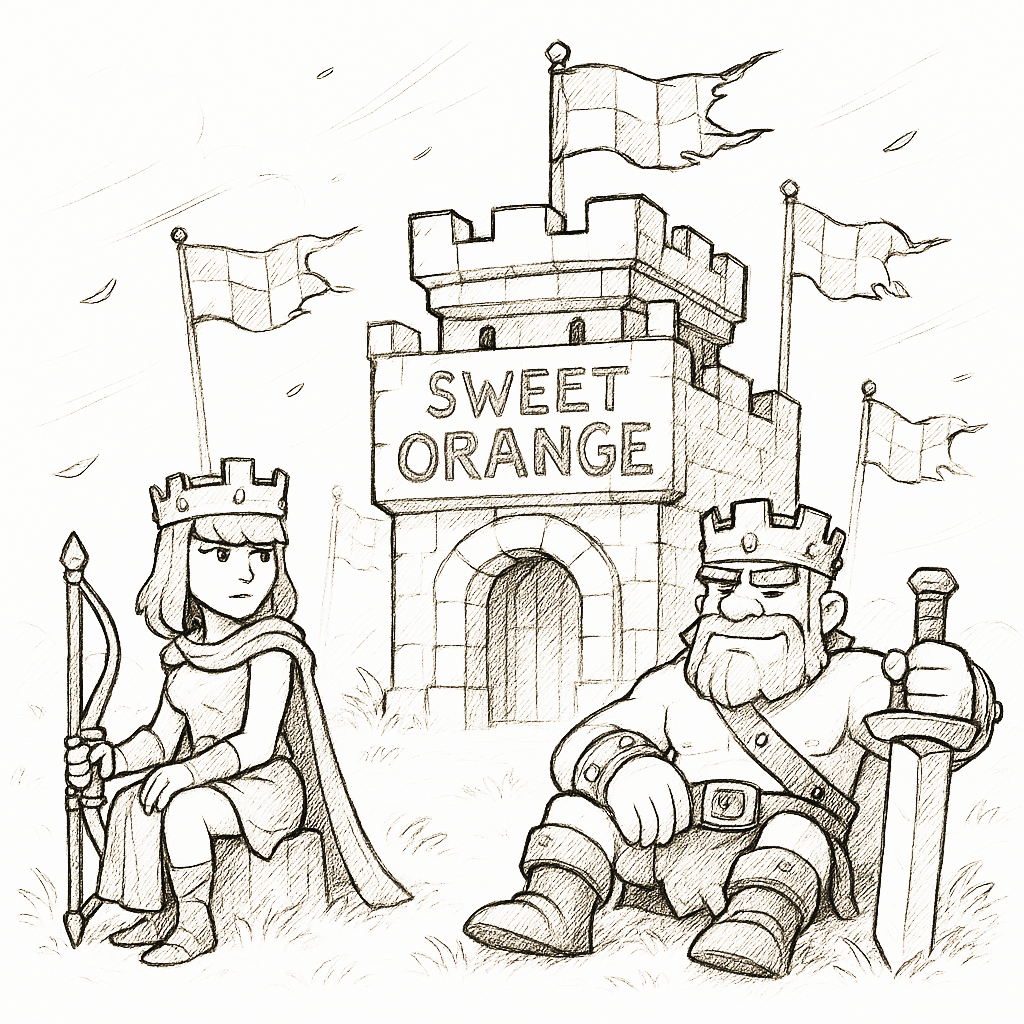
\includegraphics[width=.5\linewidth]{image/Sweet Orange Castle.jpg}
    \end{center}
    
    \item \textbf{Ber-\textit{caption} dan Dapat Dirujuk}. Anda dapat menggunakan \textit{environment} \texttt{figure}, dengan beberapa format \& opsi yang tersedia seperti:
    \begin{lstlisting}
        \begin{figure}[H]
            \centering
            \includegraphics[width=UKURAN_LEBAR]{LOKASI_FILE_GAMBAR}
            \caption{ISI_KETERANGAN}
            \label{fig:KATA_TUNJUK}
            \figuresource{SUMBER_GAMBAR}
        \end{figure}
    \end{lstlisting}
    
    \begin{figure}[H]
        \centering
        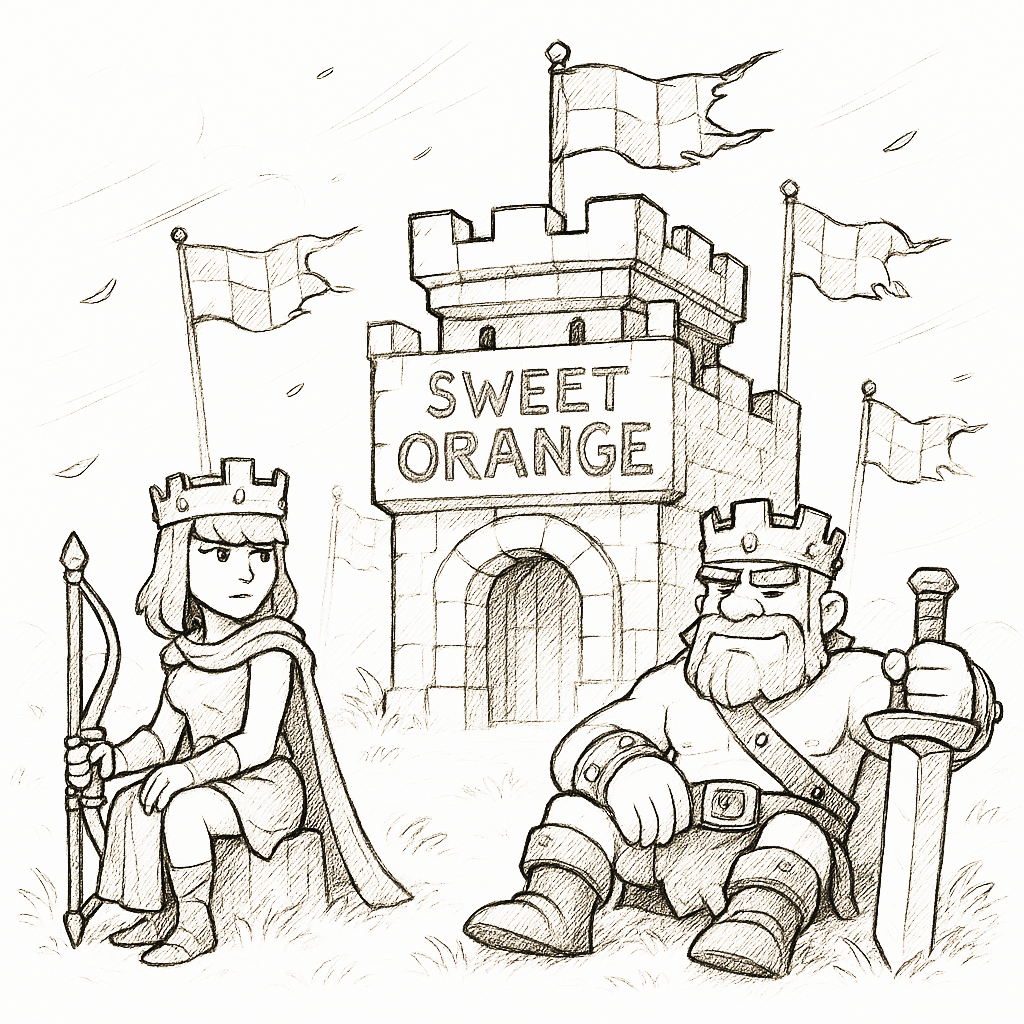
\includegraphics[width=.5\linewidth]{image/Sweet Orange Castle.jpg}
        \caption{Sketsa Raja dan Ratu Menjaga Kastel}
        \label{fig:sketsa-kastel}
        \figuresource{\url{https://sora.chatgpt.com/g/gen_01k0gx9pfrfpmtj3cb91zfg4dk}}
    \end{figure}
    
    Sekarang kita coba tunjuk. Sketsa dalam \autoref{fig:sketsa-kastel} diambil dari referensi dalam permainan Clash of Clans. Gambar dibuat dengan menggunakan akal imitasi (AI).
\end{enumerate}

\section{Tabel}

\subsection{\textit{Tabular}}

\textit{Tabular} dapat digunakan untuk membuat tabel secara sederhana. Cara pemakaian tersedia dalam situs \url{https://www.overleaf.com/learn/latex/Tables}. Tabel \textit{tabular} dapat dibuat dengan mudah melalui fitur pembantu seperti \textit{Table Wizard} bawaan TeX Studio, \textit{Tabular Generator}, atau meminta tolong kepada AI.

\begin{enumerate}[label=\alph*.]
    \item \textbf{Polosan}. Gunakan \textit{environment} \texttt{tabular}.
    \begin{center}
        \begin{tabular}{c l r}
            \hline
            No. & Provinsi & Jemaah Haji \\
            \hline
            1 & Jawa Barat & 39753 \\
            2 & Jawa Timur & 36980 \\
            3 & Jawa Tengah & 31757 \\
            4 & Banten & 10244 \\
            5 & Sumatera Utara & 8516 \\
            \hline
        \end{tabular}
    \end{center}
    
    \item \textbf{Ber-\textit{caption} dan Dapat Dirujuk}. Bungkuslah \textit{environment} \texttt{tabular} dengan \textit{environment} \texttt{table}, dengan format dan beberapa opsi seperti:
    \begin{lstlisting}[]
        \begin{table}[H]
            \centering
            \caption{KETERANGAN}
            \longcaption{KETERANGAN_BARIS_1 \\ KETERANGAN_BARIS_2}
            \label{table:KATA_TUNJUK}
            \begin{tabular}{...}
                ...
            \end{tabular}
            \tablesource{SUMBER_DATA}
            \tablesourceleft{JARAK_INDENT_KE_KANAN}{SUMBER_DATA}
        \end{table}
    \end{lstlisting}
    
    Anda harus memakai salah satu antara \verb|\caption| atau \verb|\longcaption|, demikian juga untuk \verb|\tablesource| atau \verb|\tablesourceleft|.
    
    \begin{table}[H]
        \centering
        \longcaption{Lima Provinsi dengan Jumlah Jemaah Haji Terbanyak \\ yang Diberangkatkan ke Tanah Suci Mekah (2024)}
        \label{table:5-provinsi-jemaah-haji}
        \begin{tabular}{c l r}
            \hline
            No. & Provinsi & Jemaah Haji \\
            \hline
            1 & Jawa Barat & 39753 \\
            2 & Jawa Timur & 36980 \\
            3 & Jawa Tengah & 31757 \\
            4 & Banten & 10244 \\
            5 & Sumatera Utara & 8516 \\
            \hline
        \end{tabular}
        \tablesource{\citeA{BPS-2025:jumlah-jemaah-24}}
    \end{table}
    
    Sekarang kita coba tunjuk. Data yang ditunjukkan pada \autoref{table:5-provinsi-jemaah-haji} diambil berdasarkan jumlah jemaah haji terbanyak pada wilayah tersebut. Jumlah terbanyak diletakkan di baris nomor satu.
\end{enumerate}

\subsection{\textit{Tabularray}}

\textit{Tabularray} dapat digunakan untuk membuat tabel sesuka hati --- dalam artian mudah dikustomisasi dan disetel sesuka hati. Cara penggunaan dasar dapat Anda baca melalui \url{https://www.latex-tables.com/ressources/tabularray.html} atau lebih jitu lagi dengan dokumentasi \textit{Tabularray} di \url{https://mirror.unpad.ac.id/ctan/macros/latex/contrib/tabularray/tabularray.pdf}. Tabel \textit{tabularray} dapat dibuat dengan mudah menggunakan AI. Mengapa begitu? Sebab masih jarang alat bantu yang tersedia untuk menulis tabel \textit{tabularray} --- sebagian besarnya hanya membantu untuk menulis tabel \textit{tabular}. Meski demikian, menyetel tabel \textit{tabularray} sebenarnya jauh lebih enak.

\subsubsection{Tblr}

\begin{enumerate}[label=\arabic*)]
    \item \textbf{Polosan}. Gunakan \textit{environment} \texttt{tblr}
    
    \begin{center}
        \begin{tblr}{colspec={c l r}, hline{1,2,Z}={1-Z}{solid}}
            No. & Provinsi & Jemaah Haji \\
            1 & Jawa Barat & 39753 \\
            2 & Jawa Timur & 36980 \\
            3 & Jawa Tengah & 31757 \\
            4 & Banten & 10244 \\
            5 & Sumatera Utara & 8516
        \end{tblr}
    \end{center}
    
    \item \textbf{Ber-\textit{caption} dan Dapat Dirujuk}. Bungkuslah \textit{environment} \texttt{tblr} dengan \textit{environment} \texttt{table}, dengan format dan beberapa opsi seperti:
    \begin{lstlisting}
        \begin{table}[H]
            \centering
            \caption{KETERANGAN}
            \longcaption{KETERANGAN_BARIS_1 \\ KETERANGAN_BARIS_2}
            \label{table:KATA_TUNJUK}
            \begin{tblr}{...}
                ...
            \end{tblr}
            \tablesource{SUMBER_DATA}
            \tablesourceleft{JARAK_INDENT_KE_KANAN}{SUMBER_DATA}
        \end{table}
    \end{lstlisting}
    
    Anda harus memakai salah satu antara \verb|\caption| atau \verb|\longcaption|, demikian juga untuk \verb|\tablesource| atau \verb|\tablesourceleft|.
    
    \begin{table}[H]
        \centering
        \longcaption{Lima Provinsi dengan Jumlah Jemaah Haji Terbanyak \\ yang Diberangkatkan ke Tanah Suci Mekah (2024)}
        \label{table:5-provinsi-jumlah-jemaah-24-1}
        \begin{tblr}{colspec={c l r}, hline{1,2,Z}={1-Z}{solid}}
            No. & Provinsi & Jemaah Haji \\
            1 & Jawa Barat & 39753 \\
            2 & Jawa Timur & 36980 \\
            3 & Jawa Tengah & 31757 \\
            4 & Banten & 10244 \\
            5 & Sumatera Utara & 8516
        \end{tblr}
        \tablesource{\citeA{BPS-2025:jumlah-jemaah-24}}
    \end{table}
    
    Sekarang kita coba tunjuk. Data yang ditunjukkan pada \autoref{table:5-provinsi-jumlah-jemaah-24-1} diambil berdasarkan jumlah jemaah haji terbanyak pada wilayah tersebut. Jumlah terbanyak diletakkan di baris nomor satu.
\end{enumerate}

\subsubsection{Long Tblr}

\textit{Long Tblr} dapat digunakan untuk membuat tabel yang panjang hingga lebih dari satu halaman, tetapi boleh-boleh saja jika ingin digunakan sebagai pengganti \textit{tabular} atau \textit{tblr}. Anda dapat menggunakannya dengan \textit{environment} \texttt{longtblr} disertai dengan format dan opsi seperti:
\begin{lstlisting}
    \begin{longtblr}[
        caption={KETERANGAN},
        label={table:KATA_TUNJUK},
        remark{Sumber}={SUMBER_DATA}
        ]{
            ...
        }
        ...
    \end{longtblr}
\end{lstlisting}

\begin{longtblr}[
    caption={Jumlah Jemaah Haji yang Diberangkatkan ke Tanah Suci Mekah Menurut Provinsi, 2024},
    label={table:5-provinsi-jumlah-jemaah-24-2},
    remark{Sumber}={\citeA{BPS-2025:jumlah-jemaah-24}}
    ]{colspec={c l r}, hline{1,2,Z}={1-Z}{solid}}
    No. & Provinsi & Jemaah Haji \\
    1 & Aceh & 4593 \\
    2 & Bali & 725 \\
    3 & Banten & 10244 \\
    4 & Bengkulu & 1685 \\
    5 & DI Yogyakarta & 3306 \\
    6 & DKI Jakarta & 7885 \\
    7 & Gorontalo & 999 \\
    8 & Jambi & 3051 \\
    9 & Jawa Barat & 39753 \\
    10 & Jawa Tengah & 31757 \\
    11 & Jawa Timur & 36980 \\
    12 & Kalimantan Barat & 2588 \\
    13 & Kalimantan Selatan & 4040 \\
    14 & Kalimantan Tengah & 1672 \\
    15 & Kalimantan Timur & 2716 \\
    16 & Kalimantan Utara & 436 \\
    17 & Kepulauan Bangka Belitung & 1098 \\
    18 & Kepulauan Riau & 1305 \\
    19 & Lampung & 7152 \\
    20 & Maluku & 1080 \\
    21 & Maluku Utara & 1102 \\
    22 & Nusa Tenggara Barat & 4750 \\
    23 & Nusa Tenggara Timur & 689 \\
    24 & Papua & 1070 \\
    25 & Papua Barat & 739 \\
    26 & Riau & 5252 \\
    27 & Sulawesi Barat & 1508 \\
    28 & Sulawesi Selatan & 7758 \\
    29 & Sulawesi Tengah & 2055 \\
    30 & Sulawesi Tenggara & 2098 \\
    31 & Sulawesi Utara & 711 \\
    32 & Sumatera Barat & 4780 \\
    33 & Sumatera Selatan & 7205 \\
    34 & Sumatera Utara & 8516 \\
    & Indonesia & 211298 \\
\end{longtblr}

\section{Kode Program}

Kode program dapat disipkan dengan menggunakan \texttt{lstlisting}. Anda dapat menyetelnya sesuka hati dengan beberapa opsi yang tersedia seperti:

\begin{verbatim}
    \begin{lstlisting}[
        language=BAHASA_PROGRAM, 
        numbers=left, 
        caption={KETERANGAN}, 
        label={code:KATA_TUNJUK}
        ]
        ...
    \end{lstlisting}
    \lstsource{SUMBER}
\end{verbatim}

\begin{enumerate}[]
    \item \textbf{Polosan}. Cukup gunakan \textit{environment} \texttt{lstlisting} tanpa perlu disetel.
    
    \begin{lstlisting}
        # Program 1
        
        frekuensi_game <- seq(1, 40, length.out = 100)
        peluang_tengah <- 15
        scale <- 4
        data_peluang_logistik <- 1 - plogis(frekuensi_game, peluang_tengah, scale)
        
        # Grafik
        x11()
        plot(frekuensi_game, data_peluang_logistik,
        type = "l",
        xlab = "Game/Match per Hari",
        ylab = "Peluang untuk 'Dikasih Menang'",
        yaxt = "n",
        col = "red",
        main = paste0("Peluang Kemenangan Game Online | Dist. Logistik: μ = ", peluang_tengah, ", 𝒔 = ", scale),
        sub = "(Semakin Sering Main, Semakin Rendah Peluang Kemenangannya)")
        
        axis(side = 2, at = seq(0, 1, by = 0.2), labels = paste0(seq(0, 1, by = 0.2) * 100, "%"), las = 1)
    \end{lstlisting}
    
    \item \textbf{\textit{Formatted}}. Kode program ditulis dengan menambahkan setelan. Misalnya contoh kode tersebut menggunakan bahasa R. Kode yang disetel bahasanya menjadi R, lalu ditambahkan nomor barisnya dapat terlihat seperti:
    
    \begin{lstlisting}[language=R, numbers=left]
        # Program 1
        
        frekuensi_game <- seq(1, 40, length.out = 100)
        peluang_tengah <- 15
        scale <- 4
        data_peluang_logistik <- 1 - plogis(frekuensi_game, peluang_tengah, scale)
        
        # Grafik
        x11()
        plot(frekuensi_game, data_peluang_logistik,
        type = "l",
        xlab = "Game/Match per Hari",
        ylab = "Peluang untuk 'Dikasih Menang'",
        yaxt = "n",
        col = "red",
        main = paste0("Peluang Kemenangan Game Online | Dist. Logistik: μ = ", peluang_tengah, ", 𝒔 = ", scale),
        sub = "(Semakin Sering Main, Semakin Rendah Peluang Kemenangannya)")
        
        axis(side = 2, at = seq(0, 1, by = 0.2), labels = paste0(seq(0, 1, by = 0.2) * 100, "%"), las = 1)
    \end{lstlisting}
    
    \item \textbf{Ber-\textit{caption} dan Dapat Dirujuk}. 
    
    \begin{lstlisting}[
        language=R, 
        numbers=left,
        caption={Gambaran Win/Lose Permainan dengan Grafik Logistik},
        label={code:grafik-winlose-game}
        ]
        # Program 1
        
        frekuensi_game <- seq(1, 40, length.out = 100)
        peluang_tengah <- 15
        scale <- 4
        data_peluang_logistik <- 1 - plogis(frekuensi_game, peluang_tengah, scale)
        
        # Grafik
        x11()
        plot(frekuensi_game, data_peluang_logistik,
        type = "l",
        xlab = "Game/Match per Hari",
        ylab = "Peluang untuk 'Dikasih Menang'",
        yaxt = "n",
        col = "red",
        main = paste0("Peluang Kemenangan Game Online | Dist. Logistik: μ = ", peluang_tengah, ", 𝒔 = ", scale),
        sub = "(Semakin Sering Main, Semakin Rendah Peluang Kemenangannya)")
        
        axis(side = 2, at = seq(0, 1, by = 0.2), labels = paste0(seq(0, 1, by = 0.2) * 100, "%"), las = 1)
    \end{lstlisting}
    \lstsource{Dokumen Penulis}
    
    Sekarang kita coba tunjuk. Kode program yang ditampilkan pada \autoref{code:grafik-winlose-game} merupakan program R untuk menampilkan grafik peluang menang yang menurun jika seseorang bermain \textit{game} terus-menerus.
\end{enumerate}

\section{Mengelola Daftar Pustaka}

Isi daftar referensi disimpan dalam \textit{file} \texttt{reference.bib}. Daftar referensi ditulis dengan format BibTeX atau BibLaTeX seperti contoh ini.

\begin{lstlisting}
    ENTRY_TYPE{KATA_TUNJUK,
        FIELD_OPSI={ISI},
        ...
        FIELD_OPSI={ISI}
    }
\end{lstlisting}

Anda dapat melihat sebagian kecil dari \textit{entry type} dan \textit{field} yang tersedia pada \autoref{table:entry-type-bibtex} dan \autoref{table:field-opsi-bibtex}.

\begin{longtblr}[
    caption={\textit{Entry Type} BibTeX},
    label={table:entry-type-bibtex},
    remark{Sumber}={\url{https://www.bibtex.com/format/}}
    ]{colspec={l X[l]}, hline{1,2,Z}={1-Z}{solid}, row{1}={halign=c}}
    \textbf{Jenis Entri} & \textbf{Peruntukan} \\
    @article & Digunakan untuk artikel dalam jurnal, majalah, atau koran. \\
    @book & Digunakan untuk buku yang diterbitkan dengan penulis yang jelas. \\
    @inbook & Digunakan untuk bagian dari buku, seperti bab atau esai. \\
    @booklet & Digunakan untuk dokumen cetak yang tidak memiliki penerbit atau penulis yang terikat. \\
    @collection & Digunakan untuk kumpulan tulisan yang diterbitkan sebagai satu volume (misal, kumpulan esai). \\
    @incollection & Digunakan untuk artikel atau bab dalam sebuah koleksi. \\
    @proceedings & Digunakan untuk kumpulan artikel dari konferensi. \\
    @inproceedings & Digunakan untuk artikel tunggal dalam prosiding konferensi. \\
    @manual & Digunakan untuk panduan teknis atau manual. \\
    @mastersthesis & Digunakan untuk tesis master. \\
    @phdthesis & Digunakan untuk disertasi doktoral. \\
    @online & Digunakan untuk dokumen yang diterbitkan secara daring, seperti halaman web atau blog. \\
    @report & Digunakan untuk laporan teknis yang dikeluarkan oleh institusi. \\
    @techreport & Sama seperti @report, tetapi lebih spesifik untuk laporan teknis. \\
    @unpublished & Digunakan untuk karya yang belum diterbitkan, seperti manuskrip. \\
    @misc & Digunakan untuk jenis entri apa pun yang tidak cocok dengan kategori lainnya.
\end{longtblr}

\begin{longtblr}[
    caption={\textit{Field} Opsi BibTeX},
    label={table:field-opsi-bibtex},
    remark{Sumber}={\url{https://www.bibtex.com/format/}}
    ]{colspec={l X[l] l}, hline{1,2,Z}={1-Z}{solid}, row{1}={halign=c}}
    \textbf{Opsi} & \textbf{Keterangan} & \textbf{Contoh} \\
    author & Nama penulis. & {\texttt{author=\{Nama Penulis\}} \\ \texttt{author=\{Penulis1 and Penulis2\}} \\ \texttt{author=\{\{Nama Instansi\}\}}} \\
    editor & Nama editor. & \texttt{editor=\{Nama Editor\}} \\
    title & Judul karya. & \texttt{title=\{Judul Tulisan\}} \\
    journal & Judul jurnal tempat artikel diterbitkan. & \texttt{journaltitle=\{Nama Jurnal\}} \\
    booktitle & Judul buku tempat bagian atau artikel diterbitkan. & \texttt{booktitle=\{Judul Buku\}} \\
    year & Tahun publikasi. & \texttt{year=\{2023\}} \\
    month & Bulan publikasi. & {\texttt{month=\{3\}} \\ \texttt{month=\{mar\}} \\ \texttt{month=\{Maret\}}} \\
    day & Hari publikasi. & \texttt{day=\{15\}} \\
    publisher & Nama penerbit. & \texttt{publisher=\{Nama Penerbit\}} \\
    address & Lokasi penerbitan. & \texttt{location=\{Kota\}} \\
    volume & Nomor volume jurnal atau buku. & \texttt{volume=\{10\}} \\
    number & Nomor terbitan jurnal. & \texttt{number=\{2\}} \\
    pages & Rentang halaman. & \texttt{pages=\{23--45\}} \\
    url & URL dokumen daring. & \texttt{url=\{https://example.com\}} \\
    urldate & Tanggal akses URL dokumen daring. & {\texttt{urldate=\{2024-03-15\}} \\ \texttt{urldate=\{Maret 15, 2024\}} \\ \texttt{urldate=\{15 Maret 2024\}}} \\
    doi & Digital Object Identifier (DOI) untuk dokumen digital. & \texttt{doi=\{10.xxxx/xxxx\}} \\
    note & Catatan tambahan. & \texttt{note=\{Catatan tambahan\}} \\
    abstract & Ringkasan singkat atau abstrak dari karya. & \texttt{abstract=\{Ringkasan karya\}}
\end{longtblr}

Ini adalah contoh daftar referensi dari buku ``Aljabar Linear Elementer I'' yang ditulis oleh Rasjidin Jainudin Pamuntjak dan Warsito.

\begin{lstlisting}
    @book{warsito-2022:ALE,
        author = {Rasjidin Jainudin Pamuntjak and Warsito},
        year = {2022},
        title = {{Aljabar Linear Elementer I}},
        edition = {3},
        address = {Tangerang Selatan},
        publisher = {Universitas Terbuka}
    }
\end{lstlisting}

\section{Kutipan}

\subsection{\textit{Narrative Citation}}

\textit{Narrative citation} biasanya ditulis sebagai bagian dalam kalimat. Anda dapat menggunakannya dengan perintah \verb|\citeA{KATA_TUNJUK_DAFTAR_PUSTAKA}|. Anda dapat melihat beberapa contohnya di sini.

\subsubsection{Kutipan Singkat}

Menurut \citeA{fitriani-2024:pelatihan-latex}, ``Salah satu kelebihan utama LaTeX adalah kemampuannya untuk membuat dokumen yang kompleks, seperti laporan penelitian, makalah ilmiah, dan buku teks, dengan sangat efisien dan mudah diatur. LaTeX membuat konten dokumen yang lebih terstruktur dan berkualitas.''

Menurut \citeA{fitriani-2024:pelatihan-latex}, LaTeX sangat bagus untuk menulis karya tulis dan dokumen ilmiah karena bagian-bagian isi tulisan dan lampiran dapat diatur dengan mudah.

\subsubsection{Kutipan Panjang (dengan Blockquote)}

\citeA{fitriani-2024:pelatihan-latex} bependapat bahwa:

\begin{quote}
    Saat ini, LaTeX semakin berkembang dan bertambah lengkap dan semakin kompleks. Penyempurnaan LaTeX sampai saat ini masih berlangsung. Sebagai contoh, saat ini di Jerman, LaTeX sudah digunakan secara umum di sekolah-sekolah maupun di universitas. Salah satu kelebihan utama LaTeX adalah kemampuannya untuk membuat dokumen yang kompleks, seperti laporan penelitian, makalah ilmiah, dan buku teks, dengan sangat efisien dan mudah diatur. LaTex membuat konten dokumen yang lebih terstruktur dan berkualitas.
\end{quote}

\subsection{\textit{Parenthetical Citation}}

\textit{Parenthetical citation} biasanya ditulis dengan diapit tanda kurung kemudian diletakkan pada akhir kalimat kutipan. Anda dapat menggunakannya dengan perintah \\ \verb|\cite{KATA_TUNJUK_DAFTAR_PUSTAKA}|. Anda dapat melihat contohnya di sini.



\subsubsection{Kutipan Singkat}

Salah satu kelebihan utama LaTeX adalah kemampuannya untuk membuat dokumen yang kompleks, seperti laporan penelitian, makalah ilmiah, dan buku teks, dengan sangat efisien dan mudah diatur. LaTeX membuat konten dokumen yang lebih terstruktur dan berkualitas \cite{fitriani-2024:pelatihan-latex}.

\subsubsection{Kutipan Panjang (dengan Blockquote)}

\begin{quote}
    Saat ini, LaTeX semakin berkembang dan bertambah lengkap dan semakin kompleks. Penyempurnaan LaTeX sampai saat ini masih berlangsung. Sebagai contoh, saat ini di Jerman, LaTeX sudah digunakan secara umum di sekolah-sekolah maupun di universitas. Salah satu kelebihan utama LaTeX adalah kemampuannya untuk membuat dokumen yang kompleks, seperti laporan penelitian, makalah ilmiah, dan buku teks, dengan sangat efisien dan mudah diatur. LaTex membuat konten dokumen yang lebih terstruktur dan berkualitas \cite{fitriani-2024:pelatihan-latex}.
\end{quote}

\section{Tambahan}

Gaya sitasi dalam \textit{template} ini menggunakan APA 6 yang sedikit dimodifikasi pada sebagian istilahnya, seperti:

\begin{enumerate}[nosep]
    \item ... and ... $\longrightarrow$ ... dan ...
    \item Retrieved from ... $\longrightarrow$ Diakses dari ...
    \item Retrieved ... from ... $\longrightarrow$ Diakses ... dari ...
\end{enumerate}

Jika Anda kurang menyukai penggantian sebagian istilah ini atau lebih memilih mempertahankan bahasa Inggris, Anda dapat membuka \textit{file} \texttt{variable.tex} dan menghapus semua kode yang ada dalam bagian ``ISTILAH DALAM APA 6 DAFTAR PUSTAKA''